As already mentioned in \cref{sec:theory:solutions}, due to
the coupled integro-differential structure of \cref{eq:eko/dglap}, 
solving the equations requires in practice some approximations to which we refer as different
solution strategies. \eko{} currently implements 8 different strategies,
corresponding to different approximations.
Note that they may differ only by the strategy in a specific sector,
such as the singlet or non-singlet sector. All provided strategies
agree at fixed order, but differ by higher order terms.

In \cref{fig:solutions} we show a comparison of a selected list of
solution strategies\footnote{For the full list of available solutions and a
detailed descriptions see the
\href{https://eko.readthedocs.io/en/latest}{online documentation}.}:

\begin{itemize}
    \item \texttt{iterate-exact}:
        In the non-singlet sector we take the analytical solution
        of \cref{eq:eko/dglap2} up to the order specified.
        In the singlet sector we split the evolution path into segments
        and linearize the exponential in each segment~\cite{Bonvini:2012sh}.
        This provides effectively a straight numerical solution of \cref{eq:eko/dglap2}.
        In \cref{fig:solutions} we adopt this strategy as a reference.
    \item \texttt{perturbative-exact}:
        In the non-singlet sector it coincides with \texttt{iterate-exact}.
        In the singlet sector we make an ansatz to determine the solution as a
        transformation $\vb{U}(a_s)$ of the \lo{} solution~\cite{Vogt:2004ns}. We then
        iteratively determine the perturbative coefficients of $\textbf{U}$.
    \item \texttt{iterate-expanded}:
        In the singlet sector we follow the strategy of \texttt{iterate-exact}.
        In the non-singlet sector we expand \cref{eq:eko/dglap2} first to the order
        specified, before solving the equations.
    \item \texttt{truncated}: 
        In both sectors, singlet and non-singlet, we make an ansatz to determine the solution as a
        transformation $\vb{U}(a_s)$ of the \lo{} solution and
        then expand the transformation $\vb U$ up to the order specified.
        Note that for programs using $x$-space this strategy is difficult
        to pursue as the \lo{} solution is kept exact and only the transformation
        $\vb U$ is expanded.
\end{itemize}

The strategies differ most in the small-$x$ region where the \pdf{} evolution is
enhanced and the treatment of sub-leading corrections become relevant.
This feature is seen most prominently in the singlet sector between
\texttt{iterate-exact} (the reference strategy) and \texttt{truncated}.
In the non-singlet sector the distributions also vanish for small-$x$
and so the difference gets artificially enhanced.
This is eventually the source of the spread for the valence distribution $V(x)$
making it more sensitive to the initial \pdf{}.

\begin{figure}
    \centering
    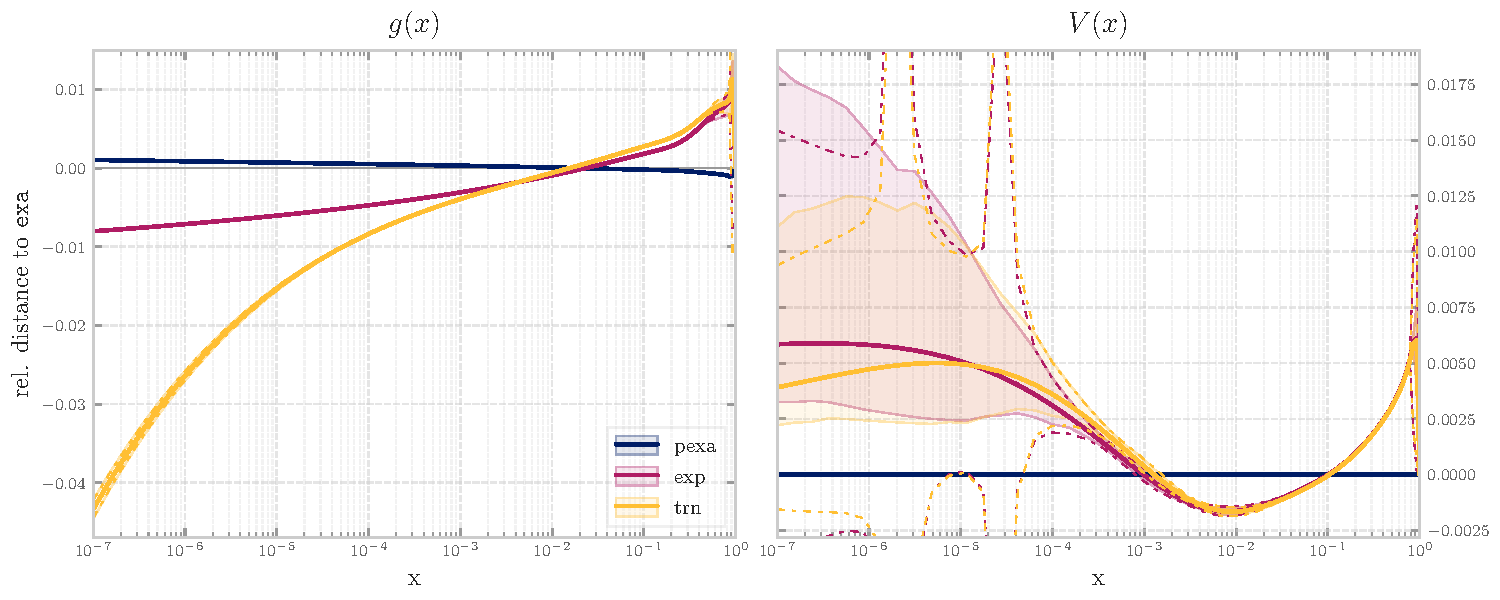
\includegraphics[width=\textwidth]{ch-eko/solutions-main}
    \caption{Compare selected solutions strategies, with respect to the
        \texttt{iterated-exact} (called \texttt{exa} in label) one. In
        particular: \texttt{perturbative-exact} (\texttt{pexa}) (matching
        the reference in the non-singlet sector),
        \texttt{iterated-expanded} (\texttt{exp}), and \texttt{truncated}
        (\texttt{trn}).
        The distributions are evolved in $\muF^2=\SI[parse-numbers=false]{1.65^2\to 10^4}{\GeV^2}$.}
    \label{fig:solutions}
\end{figure}

\paragraph{PDF plots} The \pdf{} plot shown in \cref{fig:solutions} contains
multiple elements, and its layout is in common with
\cref{fig:interpolation,fig:pdfmatching}.

All the different entries corresponds to different theory settings, and they
are normalized with respect to a reference theory setup
(e.g.\ in \cref{fig:solutions} the \texttt{iterative-exact} strategy)
and the lines correspond to the relative difference.

Furthermore, an envelope and dashed lines are displayed.
To obtain them, the full \pdf{} set is evolved, replica by replica, for each
configuration (corresponding to a single evolution operator, that is applied to
each replica in turn).
Then ratios are taken between corresponding evolved replicas, to highlight
the \pdf{} independence of \eko{} rather then any specific set-related features.
The upper and lower borders of the envelope correspond respectively
to the $0.16$ and $0.84$ quantiles of the replicas set,
while the dashed lines correspond to one standard deviation.
